\chapter{Implementation}

\section{GNS-3}

GNS3 (Graphical Network Simulator-3) software allows us to emulate complex network designs such as Cisco Router/Switch.

It enables to run real Cisco IOS images using Dynamips in the GNS3 infrastructure, and with this software, we can create complex network designs on our computer and study in more detail for exams such as Cisco Certified Network Associate (CCNA) and Cisco Certified Network Professional (CCNP), but in the context of this internship, we will exploit the GNS-3 to deploy simple network topologies and develop a simple software (preferably in Python) to remotely modify the devices operation using NETCONF.


\subsection{Appliances}
In the context of GNS3, appliances refer to pre-configured virtual network devices that can be integrated into GNS3 for network emulation and simulation purposes. These appliances are typically virtual machines (VMs) running specialized network operating systems or software, designed to replicate the behavior and functionalities of real-world networking devices.

Appliances in GNS3 are available in various forms, such as virtual routers, switches, firewalls, load balancers, and other network devices. They allow us to create complex network topologies and simulate different network scenarios without the need for physical hardware. By utilizing these virtual appliances, we can gain practical experience in network design, testing, and troubleshooting. In the case of our implementation, we will need the following appliances:


\subsubsection{Routers:}

To work with NETCONF and YANG in GNS3, we will need a virtual router that supports these protocols. One highly recommended option is the Cisco CSR 1000v, renowned for its compatibility and seamless integration with NETCONF and YANG.

The Cisco CSR1000v is a virtual router that can be utilized within the GNS3 network simulation environment. It emulates the behavior and features of physical Cisco routers, specifically the Cisco IOS XE operating system. The CSR1000v is widely recognized for its versatility, offering extensive networking capabilities and supporting various protocols (mainly NETCONF-YANG). It enables users to create virtual network topologies and experiment with network configurations, making it a valuable tool for learning, testing, and developing networking solutions in a virtual environment using GNS3.

\begin{figure}[h]
    \centering
    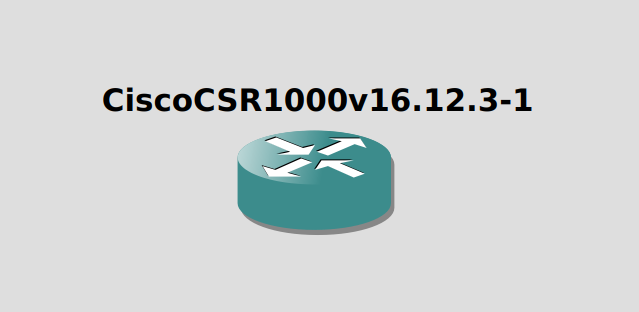
\includegraphics[width=0.7\linewidth]{Images/cisco1000v.png}
    \caption{Cisco CSR 1000v.}
    \label{fig:example}
\end{figure}

\subsubsection{Switches:}
Switches are network devices that operate at the data link layer (Layer 2) of the OSI (Open Systems Interconnection) model. They are responsible for facilitating communication between devices within a local area network (LAN). We will benefit from the key functions and features of switches:


\begin{itemize}
    \item Forwarding Frames: Switches receive network traffic in the form of frames and examine the destination MAC (Media Access Control) address of each frame. 
    \item Broadcast and Multicast Handling: Switches efficiently handle broadcast and multicast traffic within a LAN
    \item MAC Address Learning: Switches maintain a MAC address table that maps MAC addresses to specific switch ports. When a frame arrives at a switch, it checks the source MAC address and associates it with the port on which the frame was received.
\end{itemize}

\begin{figure}[h]
    \centering
    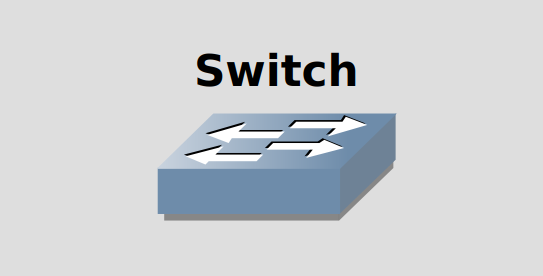
\includegraphics[width=0.7\linewidth]{Images/switch.png}
    \caption{Switch}
    \label{fig:example}
\end{figure}


\subsubsection{Virtual PC (host):}

In GNS3, a virtual PC (VPC) is a simulated computer that represents an endpoint device within a network topology. It is a virtual machine (VM) running a specific operating system that emulates the behavior and functionalities of a physical computer. Virtual PCs are used in GNS3 to simulate the interaction between network devices and end-user devices, allowing us to test and troubleshoot network configurations.

\begin{figure}[h]
    \centering
    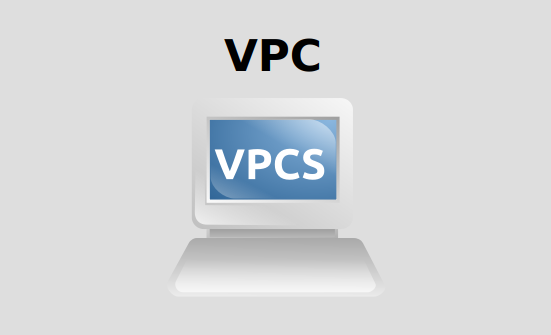
\includegraphics[width=0.6\linewidth]{Images/vpc.png}
    \caption{Virtual PC}
    \label{fig:example}
\end{figure}

\subsubsection{Cloud:}

In GNS3, the "Cloud" appliance is a versatile tool that represents external networks or connectivity points in a network topology. It allows users to establish connections between the GNS3 network and real-world networks, such as the internet or local area networks (LANs). The cloud appliance acts as a bridge between the virtual network within GNS3 and the physical network environment.

In our case, we can utilize the cloud appliance in GNS3 to connect the PC to the network. This enables the PC to function as a NETCONF administrator and perform tasks related to network management using the NETCONF protocol. Additionally, the cloud appliance can also be configured to provide Network Address Translation (NAT) functionality, allowing our virtual network in GNS3 to access resources in the external network.

\begin{figure}[h]
    \centering
    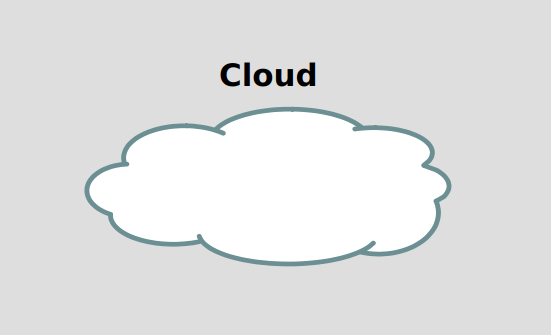
\includegraphics[width=0.5\linewidth]{Images/cloud.png}
    \caption{Cloud}
    \label{fig:example}
\end{figure}

\subsubsection{Network topology:}

Therefore, the resulting network topology will be as follows:


\begin{figure}[h]
    \centering
    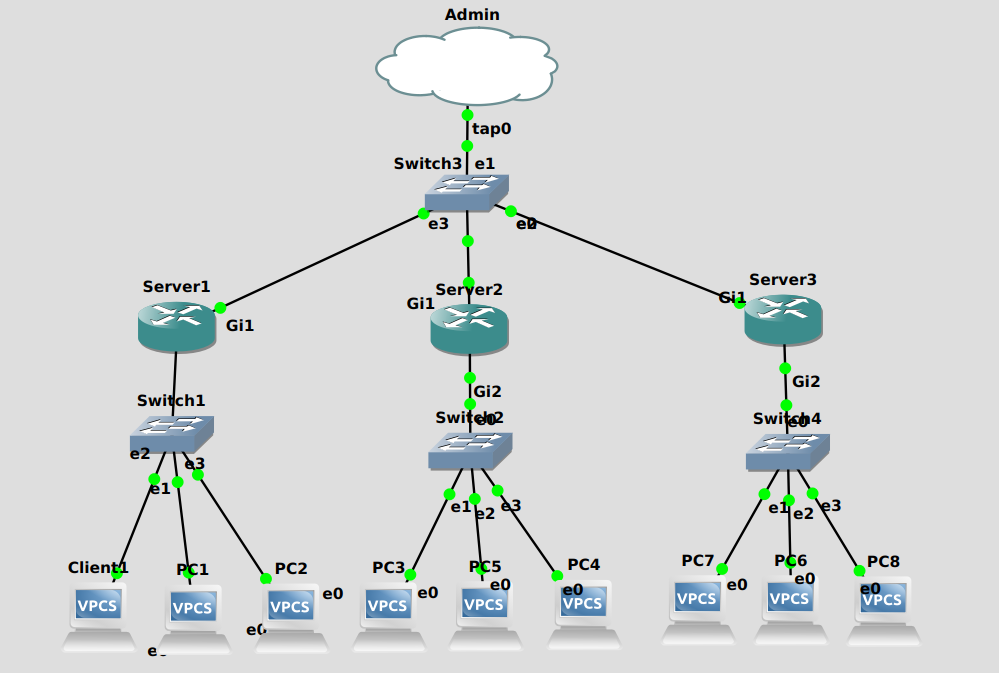
\includegraphics[width=\linewidth]{Images/network.png}
    \caption{Network topology}
    \label{fig:example}
\end{figure}
\section{Configure DHCP}
\subsection{Dynamic Host Configuration Protocol (DHCP)}
Dynamic Host Configuration Protocol (DHCP) is a client/server protocol that automatically provides an Internet Protocol (IP) host with its IP address and other related configuration information such as the subnet mask and default gateway. RFCs 2131 and 2132 define DHCP as an Internet Engineering Task Force (IETF) standard based on Bootstrap Protocol (BOOTP), a protocol with which DHCP shares many implementation details. DHCP allows hosts to obtain required TCP/IP configuration information from a DHCP server (router in our case).

Every device on a TCP/IP-based network must have a unique unicast IP address to access the network and its resources. Without DHCP, IP addresses for new computers or computers that are moved from one subnet to another must be configured manually; IP addresses for computers that are removed from the network must be manually reclaimed.

With DHCP, this entire process is automated and managed centrally. The DHCP server maintains a pool of IP addresses and leases an address to any DHCP-enabled client when it starts up on the network. Because the IP addresses are dynamic (leased) rather than static (permanently assigned), addresses no longer in use are automatically returned to the pool for reallocation.

\subsection{DHCP configuration on Cisco router:}
\subsubsection{Step 1:}
Defining the pool. The name of the pool we will give is DHCP-POOL for the subnet 10.10.10.0/24
\begin{verbatim}
    DHCP1(dhcp-config)#enable
    DHCP1(dhcp-config)#config terminal
    DHCP1(dhcp-config)#ip dhcp pool DHCP-POOL
\end{verbatim}
\subsubsection{Step 2:}
Adding the subnet that we are going to use.
\begin{verbatim}
    DHCP1(dhcp-config)#network 10.10.10.0/24
\end{verbatim}
\subsubsection{Step 3:}
Configuring the default gateway for this subnet.
\begin{verbatim}
    DHCP1(dhcp-config)#default-router 10.10.10.1
\end{verbatim}
We can also exclude the first 10 IP for manual reservations from each subnet if we are planning to add any printers or servers in the location we could use the static IP configuration from those 10 IPs later, also set a DNS server and domain, but in our case we wont need these functionalities.
%i need to include the hole code link to ANEX here

\subsubsection{Result :}
Consequently, when the end device (VPC) requests an IP address from the DHCP server (router), the client is assigned the initial IP address 10.10.10.2 :
\begin{figure}[h]
    \centering
    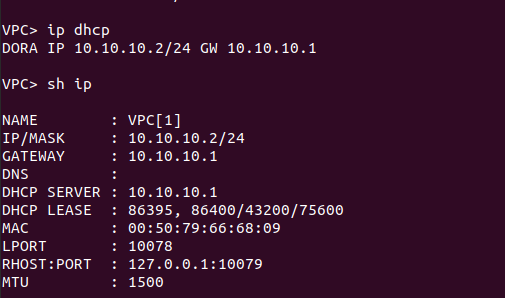
\includegraphics[width=0.7\linewidth]{Images/VPC_dhcp.png}
    \caption{IP assignment.}
\end{figure}

\section{Enabling NETCONG-YANG}

Enabling NETCONF-YANG functionality in a Cisco router is a simple process accomplished through a series of command lines entered directly into the router's console.

\begin{verbatim}
    enable 
    configure terminal
    netconf-yang
\end{verbatim}

In the case of Cisco CSR 1000v, we will need to enable candidate-datastore feature which will be discussed later:

\begin{verbatim}
    netconf-yang feature candidate-datastore
\end{verbatim}
\section{SSH connection establishment}
\subsection{Secure SHell (SSH)}
SSH, also known as Secure Shell or Secure Socket Shell, is a network protocol that gives users, particularly system administrators, a secure way to access a computer over an unsecured network.

SSH also refers to the suite of utilities that implement the SSH protocol. Secure Shell provides strong password authentication and public key authentication, as well as encrypted data communications between two computers connecting over an open network, such as the internet.

In addition to providing strong encryption, SSH is widely used by network administrators to manage systems and applications remotely, enabling them to log in to another computer over a network, execute commands and move files from one computer to another.

In our scenario, we will establish an SSH connection between the local PC, acting as an administrator, and the three routers depicted in Figure 4.5.

\subsection{Establishing an SSH connection between the router an host}
\subsubsection{On Cisco router}
\subsubsection{Step 1:}
First, we will need to configure the hostname (Ex: Server1) and domain name 
\begin{verbatim}
    hostname Server1
    ip domain-name Server1-domain
    %I need to change this 
\end{verbatim}
\subsubsection{Step 2:}
Generate rsa modulus and enter modulus lenght (2048 recommended), also configure the device to run SSHv2
\begin{verbatim}
    crypto key generate rsa modulus 2048 
    ip ssh version 
\end{verbatim}
\subsubsection{Step 3:}
Configure the virtual terminal line settings
\begin{verbatim}
    line vty 0 4 // configure the virtual terminal line settings
    login local
    transport input all
\end{verbatim}
\subsubsection{Step 4:}
Create user and password for SSH client to access, and set privilege privilege level 15 to the username ‘admin’
\begin{verbatim}
    username admin password nabil 
    username admin privilege 15 
\end{verbatim}
\indent Finaly, we don't forget to save the change by copying the ruuning configuration to the startup configuration
\subsubsection{On the local machine}
\indent First, we need to create a new virtual interface (eth1) with an automatically assigned IP address. In our case, we are using an Ubuntu machine:
\begin{verbatim}
    sudo ip link add name eth1 type dummy
    sudo ip link set eth1 up
    sudo dhclient eth1
\end{verbatim}
Following the setup, we can proceed to establish an SSH connection from the local machine, acting as the management server, to the router. The router's IP address is "192.168.1.1", and the default port for NETCONF is "830".
\begin{verbatim}
    ssh admin@192.168.1.1 -p 830 -s netconf 
    password: nabil
\end{verbatim}
\subsection{Result}









